\section{Phương pháp nghiên cứu}
\subsection{Linear Regression}
Nội dung.

% =========================================
\subsection{ARIMA}
Nội dung.
% =========================================
\subsection{RNN}
\begin{minipage}{0.45\textwidth}
\centering
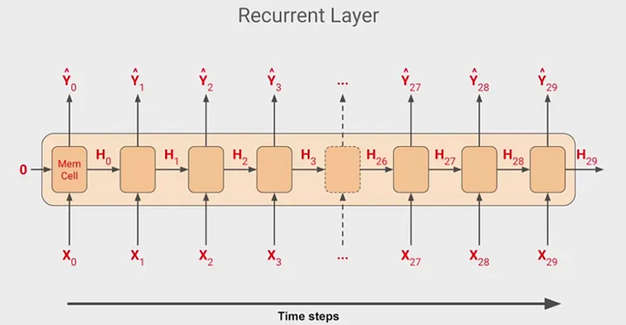
\includegraphics[width=1\textwidth]{resources/chapter-4/rnn-1.png}
\end{minipage}
\[h_t = \sigma (W_{h}x_{t} + U_h h_{t-1} + b_t) \]
\[y_t = \sigma (W_{y} h_t + b_y)\]
    \indent\textbullet\ \(h_t\): Vector lớp ẩn tại thời điểm t\\
    \indent\textbullet\ \(X_t\): vector đầu vào tại thời điểm t\\
    \indent\textbullet\ \(\widehat{Y_t}\): vector đầu ra tại thời điểm t\\
    \indent\textbullet\ \(W_h\), \(U_h\), \(W_y\): Là ma trận trọng số ngẫu nhiên\\
    \indent\textbullet\ \(b_h\), \(b_y\): là các bias\\
    \indent\textbullet\ \(\sigma_h\), \(\sigma_y\): là các hàm kích hoạt\\

Một số hàm kích hoạt phổ biến là:
\\ \textbf{Sigmoid}
\[f(x)=\frac{1}{1+e^{-x}}\]
\\ \textbf{Tanh}
\[f(x) = \frac{e^x - e^{-x}}{e^x + e^{-x}}\]
\\ \textbf{RELU}
\[f(x)=\{\begin{matrix}
0 & \text{for } x<0 \\
x & \text{for } x\ge0
\end{matrix}.\]
Thuật toán
Đầu vào: chuỗi thời gian \(x_1\), \(x_2\), \(x_3\), … \(x_t\), nhãn thực tế tương ứng \(y_1\), \(y_2\), \(y_3\), … \(y_t\),
Đầu ra: Tính toán hàm mất mát (Loss Function) và cập nhật các trọng số \(W_h\), \(U_h\), \(W_y\), \(b_h\), \(b_y\)
\[\text{Loss Function} = \frac{1}{N} \sum_{i=1}^{N} (-y_i + \hat{y_i})^2\]
Lặp lại quá trình trên cho đến khi hàm mất mát giảm đủ ( không thay đổi trong một số bước lặp nhất định, không thể giảm được nữa)
% =========================================
\subsection{LSTM}
Nội dung.

% =========================================
\subsection{GRU}
Nội dung.

% =========================================
\subsection{Kalman Filter}
Nội dung.

% =========================================
\subsection{Meta-learning}
Nội dung.

% =========================================
\subsection{NBeats}
\begin{minipage}{0.45\textwidth}
\centering
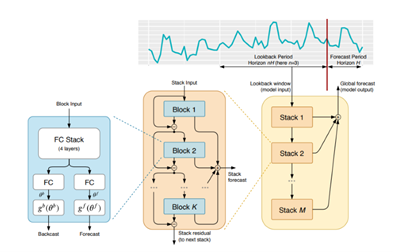
\includegraphics[width=1\textwidth]{resources/chapter-4/nbeats-1.png}
\end{minipage}
\\
\({h}_{\ell,1} = FC_{\ell,1}({x}_{\ell}), \quad {h}_{\ell,2} = FC_{\ell,2}({h}_{\ell,1}), \quad {h}_{\ell,3} = FC_{\ell,3}({h}_{\ell,2}), \quad {h}_{\ell,4} = FC_{\ell,4}({h}_{\ell,3}).\) \\
\(\theta^b_{\ell} = LINEAR_{\ell}^{b}({h}_{\ell,4}), \quad \theta^f_{\ell} = LINEAR_{\ell}^{f}({h}_{\ell,4}).\) \\

\[\widehat{\vec{y}}_{\ell} = \sum_{i=1}^{\dim(\theta^f_{\ell})} \theta^f_{\ell,i} \vec{v}^f_{i}, \quad  \widehat{\vec{x}}_{\ell} = \sum_{i=1}^{\dim(\theta^b_{\ell})} \theta^b_{\ell,i} \vec{v}^b_{i}.
\]
Mô tả cấu trúc mô hình: \\
\\
\textbf{Khối Đầu vào (Time series input)}: của mô hình là một chuỗi thời gian \(Y_{t-n+1:t}\) chứa các đặc điểm của quá khứ.\\
\textbf{Ngăn xếp khối đầu vào (Stack Input)}: cấu trúc này bao gồm các khối được xếp chống lên nhau. Mỗi khối thực hiện 2 nhiệm vụ chính là dự đoán lại quá khư (backcast) và dự báo tương lai(forecast)\\
\textbf{Broadcast}: mỗi khối cố  gắng tại tạo lại đầu vào (phần quá khứ) để dảm phần dư trước khi chuyển trang khối tiếp theo\\
\textbf{Forecast}: Mỗi khi đưa ra dự báo cho tương lai và các dự báo này được tổng hợp lại để tạo ra dự báo cuối cùng\\
\\
\textbf{Fully Connected Layers}: Mỗi khối báo gồm nhiều lớp fully-connected. Các lớp này sử dụng các hàm kích hoạt để học các bieuer diễn phi tuyến của dữ liệu\\
\textbf{Residual Connections(kết nối dư)}: sau mỗi khối, phần dư giữa đầu vào và backcast được tính toán và sử dụng làm đầu vào cho khối tiếp theo\\
\textbf{Global Forcecast}: Dự báo cuối cùng được tạo ra bằng cách tổng hợp các dự báo từ tát cả các khối. Các dự báo này được kết hợp lại để tạo ra dự báo cuối cùng cho chuỗi thời gian tương lai.\\
